% Pre-ambulo
\documentclass[a4paper, 12pt]{abnt}

%% Pacotes para texto em Inglês
% \usepackage[brazil]{babel}
% \usepackage[T1]{fontenc}
% \usepackage[latin1]{inputenc}

%% Pacotes para texto em Portugues
\usepackage[brazil]{babel}
\usepackage[utf8]{inputenc}
\usepackage[T1]{fontenc}

\usepackage{dsfont}
\usepackage{amssymb,amsmath}
\usepackage{multirow}
\usepackage[alf]{abntcite}
\usepackage[pdftex]{color, graphicx}
\usepackage{colortbl}
\usepackage{url}
\usepackage{abnt-alf}
\usepackage{abntcite}
\usepackage{algorithm}
\usepackage{algorithmic}
%% \usepackage{alg}
\usepackage{hyperref}


% Redefinicao de instrucoes
\floatname{algorithm}{Algoritmo}
\renewcommand{\algorithmicrequire}{\textbf{Entrada:}}
\renewcommand{\algorithmicensure}{\textbf{Saída:}}
\renewcommand{\algorithmicend}{\textbf{fim}}
\renewcommand{\algorithmicif}{\textbf{se}}
\renewcommand{\algorithmicthen}{\textbf{então}}
\renewcommand{\algorithmicelse}{\textbf{senão}}
\renewcommand{\algorithmicfor}{\textbf{para}}
\renewcommand{\algorithmicforall}{\textbf{para todo}}
\renewcommand{\algorithmicdo}{\textbf{faça}}
\renewcommand{\algorithmicwhile}{\textbf{enquanto}}
\renewcommand{\algorithmicloop}{\textbf{loop}}
\renewcommand{\algorithmicrepeat}{\textbf{repetir}}
\renewcommand{\algorithmicuntil}{\textbf{até que}}
\renewcommand{\algorithmiccomment}[1]{\% #1}


% Definicao da lista de simbolos
% \simb[entrada na lista de simbolos]{simbolo}:
% Escreve o simbolo no texto e uma entrada na lista de simbolos.
% Se o parametro opcional e omitido, usa-se o parametro obrigatório.
\newcommand{\simb}[2][]
{%
	\ifthenelse{\equal{#1}{}}
	{\addcontentsline{los}{simbolo}{#2}}
	{\addcontentsline{los}{simbolo}{#1}}#2
}
% Para aceitar comandos com @ (at) no nome
\makeatletter
% \listadesimbolos: comando que imprime a lista de símbolos
\newcommand{\listadesimbolos}
{
	\pretextualchapter{Lista de símbolos}
	{\setlength{\parindent}{0cm}
	\@starttoc{los}}
}
% Como a entrada sera impressa
\newcommand\l@simbolo[2]{\par #1}
\makeatother


% Definicao da lista de abreviaturas e siglas
% \abrv[entrada na lista de símbolos]{abreviatura}:
% Escreve a sigla/abreviatura no texto e uma entrada na lista de abreviaturas e siglas.
% Se o parametro opcional e omitido, usa-se o parametro obrigatorio.
\newcommand{\abrv}[2][]
{%
	\ifthenelse{\equal{#1}{}}
	{\addcontentsline{loab}{abreviatura}{#2}}
	{\addcontentsline{loab}{abreviatura}{#1}}#2
}
% Para aceitar comandos com @ (at) no nome
\makeatletter
% \listadeabreviaturas: comando que imprime a lista de abreviaturas e siglas
\newcommand{\listadeabreviaturas}
{
	\pretextualchapter{Lista de abreviaturas e siglas}
	{\setlength{\parindent}{0cm}
	\@starttoc{loab}}
}
% Como a entrada sera impressa
\newcommand\l@abreviatura[2]{\par #1}
\makeatother


% \listofalgorithms: comando que imprime a lista de algoritmos
\renewcommand{\listalgorithmname}{Lista de algoritmos}


% Hifenizacao de palavras feita de forma incorreta pelo LaTeX
\hyphenation{PYTHON ou-tros}


\titulo{Relatório técnico de desenvolvimento da biblioteca Mirobot-Poti}
\autor{Mateus Oliveira Costa Bezerra}
\orientador[Orientador]{\par Leonardo Ataide Minora, Mestre}

% Inicio do documento
\begin{document}

	\frenchspacing

	% Capa (arquivo Includes/Capa.tex)
	% Capa
% Prote��o externa do trabalho e sobre a qual se imprimem as informa��es indispens�veis 
% � sua identifica��o.

% Especifica��o da capa
\begin{titlepage}
	\begin{center}
		
		  
		\begin{minipage}{11.15cm}
			\begin{center}
				\begin{espacosimples}
					{\small \ \\
                       \textsc{Instituto Federal do Rio Grande do Norte}
                       \\
							  \textsc{Campus Natal - Central}					\\
							  \textsc{Diretoria de Gestão e Tecnologia da Informação}	   
							  \\
							  \textsc{Tecnologia em Análise e Desenvolvimento de Sistemas}}   	
                       \\
				\end{espacosimples}
			\end{center}
		\end{minipage}

			
		\vspace{6cm}
						
		% T�tulo do trabalho
		{\setlength{\baselineskip}%
		{1.3\baselineskip}
		{\LARGE \textbf{Título do trabalho}}\par}
			
		\vspace{3cm}
			
		% Nome do aluno (autor)
		{\large \textbf{Mateus Oliveira Costa Bezerra}}
						
		\vspace{6cm}
		
		% Local da institui��o onde o trabalho deve ser apresentado e ano de entrega do mesmo
		Natal-RN\\ Janeiro de 2017
	\end{center}
\end{titlepage}


	% Folha de rosto (arquivo extra-includes/FolhaRosto.tex)
	% Folha de rosto
% Cont�m os elementos essenciais � identificação do trabalho.

% T�tulo, nome do aluno e respectivo orientador e filiação
\titulo{\Large{Título}}
\autor{Nome completo do autor}
\orientador[Orientador]{\par Nome completo do orientador e titulação}
\instituicao
{
   TADS -- Curso de Tecnologia em Análise e Desenvolvimento de
   Sistemas\par 
   DIATINF -- Diretoria Acadêmica de gestão e Tecnologia da Informação\par 
   CNAT -- Campus Natal - Central\par 
   IFRN -- Instituto Federal do Rio Grande do Norte }
	
% Natureza do trabalho (não deve ser modificada)
\comentario
{
	Trabalho de conclusão de curso de graduação do curso de Tecnologia e Análise em
	Desenvolvimento de Sistemas da Diretoria de Gestão e Tecnologia de Informação
	do Instituto Federal do Rio Grande do Norte como requisito parcial para a
	obtenção do grau de Tecnologo em Análise e Desenvolvimento de
	Sistemas.\bigskip\\
   \textit{Linha de pesquisa}:\\Nome da linha de pesquisa
}
		
% Local e data
\local{Natal-RN}
\data{Mês e ano}
	
\folhaderosto

	% Folha de aprovacao (arquivo extra-includes/FolhaAprovacao.tex)
	% Folha de aprovacao
\begin{folhadeaprovacao}
	\setlength{\ABNTsignthickness}{0.4pt}
	\setlength{\ABNTsignwidth}{10cm}

	\noindent
	Trabalho de Conclusão de Curso de Graduação sob o título
	\textit{\ABNTtitulodata} apresentada por Nome completo do autor e aceita pelo Diretoria
	de Gestão e Tecnologia da Informação do Instituto Federal do Rio Grande do
	Norte, sendo aprovada por todos os membros da banca examinadora abaixo especificada:

	% Membros da banca examinadora e respectivas filiacoes
	\assinatura
	{
		Leonardo Ataide Minora, Mestre   			                  \\
		{\small Presidente}											          \smallskip\\
		{\footnotesize
			DIATINF -- Diretoria Acadêmica de Gestão e Tecnologia da Informação		   \\
		  	IFRN -- Instituto Federal do Rio Grande do Norte
		}
   }

   \assinatura
	{
      Nome completo do examinador e titulação   			                  \\
		{\small Examinador}											          \smallskip\\
		{\footnotesize
			Diretoria/Departamento		\\
		  	Instituto
		}
   }

   \assinatura
	{
      Nome completo do examinador e titulação   			                  \\
		{\small Examinador}											          \smallskip\\
		{\footnotesize
			Diretoria/Departamento		\\
		  	Universidade
		}
	}

	\vfill

	\begin{center}
		Natal-RN, data da defesa (dia, mês e ano).
	\end{center}
\end{folhadeaprovacao}


	% Dedicatoria (arquivo extra-includes/Dedicatoria.tex)
	%% Dedicat�ria

\chapter*{}
\vspace{15cm}
\begin{flushright}
	Homenagem que o autor presta a uma ou mais pessoas.
\end{flushright}

	% Agradecimentos (arquivo extra-includes/Agradecimentos.tex)
	%% Agradecimentos

\chapter*{Agradecimentos}

Agradecimentos dirigidos àqueles que contribuíram de maneira relevante à
elaboração do trabalho, sejam eles pessoas ou mesmo organizações.


   % Epigrafe (arquivo extra-includes/Epigrafe.tex)
	% Ep�grafe (cita��o seguida de indica��o de autoria)

\chapter*{}
\vspace{15cm}
\begin{flushright}
	\textit
	{
		Citação
	}\medskip\\ 
	Autor
\end{flushright}

	% Resumo em l���ngua vernacula (arquivo extra-includes/Resumo.tex)
	% Resumo
\begin{center}
	{\Large{\textbf{\ABNTtitulodata}}}
\end{center}

\vspace{1cm}

\begin{flushright}
  Autor: \ABNTautordata\\
  Orientador(a): Leonardo Ataide Minora, Mestre
\end{flushright}

\vspace{1cm}

\begin{center}
	\Large{\textsc{\textbf{Resumo}}}
\end{center}

\noindent O aumento de interesse pela área da programação voltada para jovens e
crianças vem com o aumento da necessidade de novas estratégias e metodologias
de ensino que se adequem a esse público. Além dessa necessidade, existe a
necessidade de meios alternativos para o ensino de programação nos cursos
superiores e técnicos, principalmente no contexto brasileiro já que a área de
informática esta diretamente ligado à língua inglesa, na qual nem todos os
alunos falantes do português tem domínio. Seguindo esses dois contextos nasce a
proposta desse trabalho, que é juntar uma forma alternativa de ensino de
programação, chamada de programação tangível, a qual nasceu para ser voltada ao
ensino de programação para prianças; com uma linguagem de programação em
português desenvolvida para o ensino de lógica de programação, o potigol. Essa
junção vai ser feita através da construção de uma biblioteca para a linguagem
potigol, que possibilite programar as ações de um robô chamado de mirobot.

\noindent\textit{Palavras-chave}: programação tangível, potigol, mirobot.


	% Abstract, resumo em l���ngua estrangeira (arquivo Include/Abstract.tex)
	% Resumo em l�ngua estrangeira (em ingl�s Abstract, em espanhol Resumen, em franc�s R�sum�)
\begin{center}
	{\Large{\textbf{Título do trabalho (em língua estrangeira)}}}
\end{center}

\vspace{1cm}

\begin{flushright}
	Author: Mateus Oliveira Costa Bezerra\\
	Supervisor: Leonardo Ataide Minora, Mestre
\end{flushright}

\vspace{1cm}

\begin{center}
	\Large{\textsc{\textbf{Abstract}}}
\end{center}

\noindent O resumo em língua estrangeira (em inglês \textit{Abstract}, em
espanhol \textit{Resumen}, em francês \textit{Résumé}) é uma versão do resumo
escrito na língua vernícula para idioma de divulgação internacional. Ele deve
apresentar as mesmas características do anterior (incluindo as mesmas palavras,
isto é, seu conteúdo não deve diferir do resumo anterior), bem como ser seguido
das palavras representativas do conteúdo do trabalho, isto é, palavras-chave
e/ou descritores, na língua estrangeira. Embora a especificação abaixo considere
o inglês como língua estrangeira (o mais comum), não fica impedido a adoção de
outras linguas (a exemplo de espanhol ou francês) para redação do resumo em
língua estrangeira.

\noindent\textit{Keywords}: Keyword 1, Keyword 2, Keyword 3.


	% Lista de figuras
%	\listoffigures

	% Lista de tabelas
%	\listoftables

	% Lista de abreviaturas e siglas
%	\listadeabreviaturas

	% Lista de símbolos
%	\listadesimbolos

	% Lista de algoritmos (se houver)
	% Devem ser incluidos os pacotes algorithm e algorithmic
% \listofalgorithms

	% Sumario
	\sumario

	% Parte central do trabalho, englobando os cap��tulos que constituem o mesmo
	% Os referidos cap��tulos devem ser organizados dentro do diret��rio "Cap��tulos"

	% Capitulo 1: Introdução (arquivo Includes/Introducao.tex)
	% Introdução
\chapter{Introdução}\label{cap:introducao}

A introdução é a parte inicial do texto e que possibilita uma visão geral de
todo o trabalho, devendo constar a delimitação do assunto tratado, objetivos da
pesquisa, motivação para o desenvolvimento da mesma e outros elementos
necessários para situar o tema do trabalho.


\section{Objetivos}

Nesta seção são definidos os objetivos gerais e específicos do trabalho.


\subsection{Objetivos Gerais}

Este trabalho tem por objetivo geral implementar uma biblioteca que permita programar na linguagem Potigol comportamentos de robôs Mirobot.

\subsection{Objetivos Específicos}

Fazem parte dos objetivos específicos deste trabalho:

\begin{itemize}
  \item Descrever o protocolo de troca de mensagens do robô Mirobot;
  \item Implementar exemplo na linguagem Potigol de programação de comportamento de robôs Mirobot;
  \item \ldots
\end{itemize}


\section{Metodologia}

Na metodologia é descrito o método de investigação e pesquisa para o
desenvolvimento e implementação do trabalho que está sendo proposto.

1. Entendeu o funcionamento do robô através das ferramentas "página web" e "simulador do Mirobot"
2. Definiu os métodos (assinaturas) de programação do robô através do estudo da implementação de biblioteca "Python"
3. Testou a importação de bibliotecas no Potigol
4. Implementou o exemplo de programação em potigol de comportamento do Mirobot
5. Implementou as assinaturas
6. Criou e testou outros exemplos

\section{Delimitação do trabalho}

Devido a dificuldades na importação do robô, foi utilizado o simulador.


\section{Organização do trabalho}

Nesta seção deve ser apresentado como está organizado o trabalho, sendo
descrito, portanto, do que trata cada capítulo.
O trabalho esta organizado na seguinte estrutura: o \hyperref[cap:introducao]{primeiro capítulo}, com uma introdução sobre o trabalho; o \hyperref[cap:refencial]{segundo capítulo} com referencial teórico utilizado, descrição da implementação e teste, considerações finais.


	% Capitulo 2: Segundo capítulo (arquivo Includes/Capitulo2.tex)
	% Capítulo 2
\chapter{Mirobot e Potigol: tecnologias alternativas para o ensino de programação}
\label{cap:referencial}

\section{Mirobot: uma proposta de uso de robôs para ensino de lógica de
programação}
\label{sec:mirobot}

Um dos principais objetivos da programação tangível é tornar o que é complexo e
virutal em algo simples que pode ser visto e manuseado facilmente no mundo
real~\cite{Horn2008, Horn2007, McNerney2000}. Esse mesmo pensamento pode ser estendido da seguinte forma: durante o aprendizado de programação é comum que os alunos apliquem seus
conhecimentos para manipular recursos virtuais como: números, cadeias de
caracteres (strings) e valores booleanos. 
Como forma de alternativa ao uso dos
objetos virtuais, existe a possibilidade de se usar robôs e programar as suas
ações. 
Tenta-se com isso tornar mais intuitivo para visualizar e aprender a
lógica de programação, principalmente para crianças, pois os resultados dos
seus programas serão mostrados em um mundo real e não em uma tela de computador.

Devido a esse cenário, a empresa Google desenvolveu o Mirobot. O Mirobot é em um robô
cujas ações podem ser programadas tanto através das
linguagens de programação: Scratch, Javascript e Python; como também através um módulo que
também implementa a noção de programação tangível chamado \textit{Project Bloks}. 
A proposta do mirobot é ser um robô que recebe comandos de uma determinada fonte
via Wi-Fi e ao realizar essas ações ele vai marcando o seu trajeto com uma
caneta, resultando em um desenho.
Entre as principais ações que ele realiza
estão: se movimentar para frente ou para atrás, girar para esquerda ou para
direita, descer ou levantar a caneta (possibilitando com que ele desenhe ou não
seu trajeto quando desejado).


\subsection{Resumo da arquitetura do Mirobot}

% hardware microcontrolador, motor parágrafo para explicar a parte física do
% mirobot.

O Mirobot é composto basicamente por um chassi de madeira que é formado por:
duas rodas responsáveis pela sua movimentação, uma terceira roda no formato
esférico (que ajuda na sustentação e movimentação do robô) e um orifício onde é
possível fazer o encaixe de uma caneta.
Já na parte dentro do seu corpo,
existem dois motores de passo, cada um responsável por uma das rodas, os quais
são encarregados pela sua movimentação. 
Além desses dois motores, ainda há um
servomoto que fica responsável pelo acionamento da caneta. 
Na parte de controle
ele contém um arduíno nano responsável pelo acionamento dos motores, e a
comunicação via Wi-Fi e o tratamento dos dados fica por conta de um controlador
principal, o qual é desenvolvido pela mesma empresa do mirobot.

% parágrafo para explicar a parte comunicação do mirobot.
% software websocket
A comunicação com o Mirobot é feita via Wi-Fi e ele trabalha com a tecnologia
chamada websocket ~\cite{websocket2011}. O websocket consiste em uma tecnologia que oferece um meio
de comunicação bidirecional através de um único soquete, essa tecnologia
normalmente é usada em browsers web e servidores web. 
As mensagens que são
enviadas e recebidas pelo Mirobot estão no formado JSON (Javascript Object
Notation).

Todo esse projeto é mantido em um repositório no portal Github nos endereços: chassi em \url{https://github.com/mirobot/mirobot-chassis}; firmware arduino em \url{https://github.com/mirobot/mirobot-arduino} e o firmware wifi em \url{https://github.com/mirobot/mirobot-wifi}.

\subsection{Códigos e projetos do Mirobot}
\label{subsec:mirobotcodigos}

% Projetos que estão no Github

O Mirobot é rodeado por um grande ecossistema de projetos relacionados a ele no
repositório Github (\url{https://github.com/mirobot}), entre eles estão:

\begin{itemize}
    \item \textit{mirobot-sim}, que é um simulador
que tem a função de receber as mensagens em JSON via websocket e simular a
parte de comunicação do robô;
    \item \textit{mirobot-py}, \texit{mirobot-js} e \texit{mirobot-scratch} que são
bibliotecas para o controle do mirobot para as respectivas linguagens Python,
Javascript e Scratch;
\end{itemize}

Além dos projetos no Github ainda existe uma gama de aplicativos web com
plataformas de interação com o mirobot, podem ser encontradas em:
\url{http://apps.mirobot.io/}. Para cada uma das linguagens de programação há uma aplicação web que possibilita comunicação com o robô, em todas
essas aplicações, além da possibilidade de se conectar com o robô físico e
enviar os comandos, é possível acompanhar o seu trajeto por meio de um
simulador.  Ainda existem outros aplicativos relacionados a comunicação com o
mirobot, entre eles estão: point \& click, que é uma interface para definir o
trajeto do mirobot apenas usando clicks na tela de um simulador; e remote
control, que atua como um remoto possibilitando o envio das ações para o
mirobot por meio de botões na interface web.

\section{Linguagem Potigol uma linguagem em português para o ensino de lógica
de programação de computadores}
\label{sec:potigol}

No ano de 2011 no Instituto Federal de Educação, Ciências e Tecnologia (IFRN),
Campi Natal/Central (CNAT), foi iniciado o projeto da linguagem de programação
Potigol pelo professor Leonardo Reis Lucena e alunos bolsistas. A linguagem
nasceu com a proposta principal de auxiliar o ensino das disciplinas de
programação de computadores, e leva como principal característica a sua sintaxe
em português. Entre algumas outras características da linguagem estão: multiparadigma, tipagem estática com inferência de tipos, projetada para ser
usada por alunos iniciantes.

Atualmente a linguagem Potigol com tutorial e seus softwares utilitários estão disponíveis em \url{http://potigol.github.io} e seus projetos com seus códigos-fontes em \url{https://github.com/potigol/}.

%% Adicionar exemplo do potigol.
%% falta as referências sobre o potigol
%% 


	% Capitulo 3: Terceiro capítulo (arquivo Includes/Capitulo3.tex)
	% Capítulo 3

\chapter{Desenvolvimento da biblioteca mirobot-poti}
\label{cap:descricao}
% breve descrição da estrutura do capítulo
% url do github contendo o projeto

Este capítulo está dividido em quatro seções, as quais simboliza as etapas do
desenvolvimento da biblioteca mirobot-poti. A primeira seção descreve o protocolo de funcionamento
do mirobot e a definição da classe mirobot, assim como os seus métodos. A
segunda seção, apresenta o processo de
implementação da biblioteca e, após o seu desenvolvimento exemplificar com um
caso de uso a usando o potigol. A terceira seção descreve a parte de empacotamento do projeto. A quarta seção finaliza com exemplos de
código e testes da implementação. O código do projeto que foi desenvolvida está disponível em:
\url{https://github.com/ensino-de-programacao/mirobot-potigol}.

\section{Definição dos métodos}
\label{sec:definicao}
% descrição do protocolo de comunicação
% Definição da classe Mirobot e dos seus métodos
O início do desenvolvimento do mirobot-poti se baseou principalmente na
biblioteca mirobot-py
(\url{https://github.com/mirobot/mirobot-py}). O mirobot-py contém
os artifícios necessários para se comunicar com mirobot por meio da linguagem
Python, esse código se baseia em uma classe principal que representa o robô
mirobot e seus métodos (ações).

\begin{figure}[H]
\centering
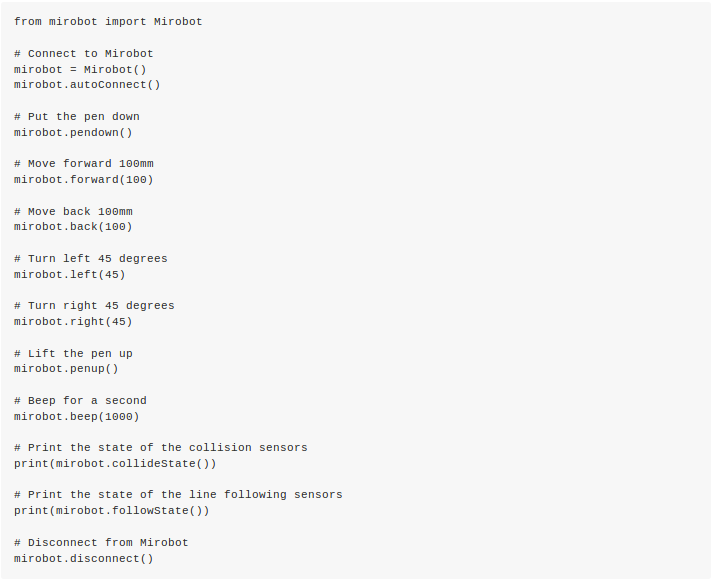
\includegraphics[scale=0.45]{imagens/desc-api.png} 
\label{fig:descapi}
  \textsf{\caption{Definição de alguns métodos da classe principal do
  mirobot-py.}}
\end{figure}

Como pode ser visto na Figura 1, esses são os métodos da classe Mirobot. Dentre eles estão os que têm o propósito de se conectar com o robô: tanto
automaticamente, por meio de uma detecção automática dos dispositivos mirobot;
quanto manualmente, inserindo o endereço IP do robô e a porta de comunicação
desejada; e por último um método para se desconectar e fechar a conexão
WebSocket. Além dos métodos de conexão, ainda tem os de movimentação, e entre
eles estão: a movimentação para trás e para frente (medida em milímetros),
movimentação para os lados (girar sobre o próprio eixo usando o grau como
medida) direito e esquerdo, e a ação ``beep'' que recebe um valor em segundos
da duração do som, por último, descer e levantar a caneta. E para finalizar, os
métodos que são responsáveis por: informar a velocidade em que os pacotes estão
sendo enviados e recebidos via Wi-Fi (ping), retorna as informações captadas
pelo sensor de colisão, retornar as informações captadas pelo sensor de
seguimento de linha.

Baseando-se nessas definições, foi criado a classe Mirobot e seus métodos na
linguagem Java. Para poder seguir o padrão do potigol, os nomes dos métodos
foram traduzidos do inglês para o português. Depois de finalizada a etapa de
definição dos métodos foi passado para a etapa de implementação. 

\section{Implementação dos métodos}
\label{sec:implementacao}
% Descrever a implementação
% Exemplo em potigol

A implementação da biblioteca mirobot-poti, foi feita através da linguagem Java.
Para a comunicação via websocket foi usado o projeto
Glassfish Tyrus(\url{https://tyrus.java.net/}). O critério de escolha pelo
Glassfish Tyrus foi devido a possibilidade de usar um servidor \textit{standalone}, ou
seja, um servidor que roda dentro da própria aplicação, caso contrário seria
necessário um servidor externo para abrigar a aplicação. 

Primeiramente foi estudado o funcionamento da biblioteca tyrus e feito alguns
exemplos simples de comunicação websocket. Depois de entendido a parte básica,
foi seguido o próximo passo de criação de um socket handler. O websocket
handler é o responsável por enviar e receber as mensagens do mirobot, ele
representa o baixo nível de comunicação e está diretamente ligado ao websocket.
As mensagens enviadas e recebidas pelo socket handler são no formato JSON (Java
Object Notation), e seguem a seguinte estrutura:

\begin{figure}[H]
\centering
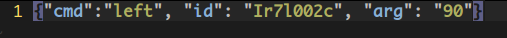
\includegraphics[scale=0.50]{imagens/comandojson.png} 
\label{fig:comandojson}
  \textsf{\caption{Exemplo de comando no formato JSON.}}
\end{figure}

Como pode ser visto na Figura 2, as mensagens JSON que são enviadas do mirobot se
baseiam em três informações: o ``cmd'' que representa o comando desejado que o
mirobot realize; o ``id'' que representa a identificação da mensagem que foi
enviada (posteriormente vai ser explicado a sua utilidade); e o ``arg'' que
representa o argumento que vai ser passado ao comando, se o comando não
precisar de argumento, como é o caso do comando usado para descer a caneta ou
de verificar o ping, esse atributo é ignorado. Então basicamente o
funcionamento da biblioteca em linhas gerais, se resume em traduzir um comando
para o formato JSON e enviá-lo via websocket obedecendo a estrutura
exemplificada na Figura 2. 

O mirobot a cada comando recebido retorna uma mensagem em JSON para informar a
situação da execução do comando recebido. O atributo ``id'' serve para identificar o comando o qual o mirobot está
informando a situação. Outro ponto importante é que, alguns comandos do mirobot
demoram mais para ser executados que outros, dependendo do tamanho do
argumento. Para exemplificar essa questão temos que levar em conta o seguinte
fator, se for enviado um comando para que o mirobot ande 10 mm para frente, ele
irá demorar um certo tempo para poder se deslocar os 10 mm, já se for enviado o
mesmo comando mudando o argumento para 20 mm, o mirobot vai demorar o dobro de
tempo para completar o percurso. 

Considerando que o mirobot não empilha as mensagens recebidas, e executa apenas
uma por vez, fica a cargo da biblioteca fazer esse controle, pois se o robô
receber um comando enquanto estiver no meio da execução de outro, irá ocorrer
um erro. A estratégia usada para resolver esse problema foi a seguinte:
todos os comandos que serão enviados para o mirobot são guardados em uma fila,
e vão sendo enviados à medida que o tempo estimado de duração de um comando
simples seja cumprido, já no caso dos comandos que têm variação de duração em
decorrer do tamanho do argumento passado, usa-se esse mesmo argumento e o
comando enviado para se estimar o tempo que vai ser esperado até o envio do
próximo comando da fila.
 
Depois de completa esses passos, foi incorporado a classe mirobot o \texit{WebsocketHandler}, o qual é usado por todos os seus métodos já
definidos anteriormente. Depois de finalizada essa etapa foi gerado o arquivo
da biblioteca, importado e testado no Potigol.

\section{O Potigol e o empacotamento da biblioteca}
\label{sec:empacotamento}
% Empacontando o projeto

Em paralelo com o desenvolvimento da biblioteca mirobot-poti, foi testado a
importação do formato jar do Potigol, todas as tentativas iniciais foram sem
sucesso pois o Potigol não conseguia fazer a importação do arquivo jar. Depois
de muitas tentativas foi descoberto que o class-path do Potigol não adicionava
os arquivos jar automaticamente, pois apesar de incluso no class-path o
diretório no qual o arquivo jar se encontrava, só era achado dentro do diretório
os arquivos class. O problema foi solucionado descompactando o arquivo jar no diretório
principal do Potigol. Outra forma que daria para resolver esse problema seria adiconando
manualmente o caminho completo do arquivo jar no class-path.

No momento de compilação do projeto mirobot-poti utilizando o maven para
automatizar a compilação, foi usado um plugin do maven chamado
``jar-with-dependences'' para que na hora da compilação as dependências do
projeto (Glassfish Tyrus) seja inserido dentro do arquivo jar, possibilitando
que o projeto após compilado dependa apenas de um único arquivo jar para ser
executado.

\section{Teste da implementação com exemplo de código}
\label{sec:testemirobot}

A última etapa do trabalho ficou com o teste na linguagem Potigol usando a
biblioteca mirobot-poti para se comunicar com o simulador do robô
(mirobot-sim). O para a realização do teste foi usado uma adaptação na classe
mirobot, pois não foi encontrado uma forma de instanciar um novo objeto dentro
do Potigol. Essa adaptação foi o uso do padrão singleton para, a qual a classe
fica responsável por gerar uma instancia da classe e retornar a variável no
Potigol. Após a implementação do teste, foi completa a etapa de desenvolvimento
do trabalho.

\begin{figure}[H]
\centering
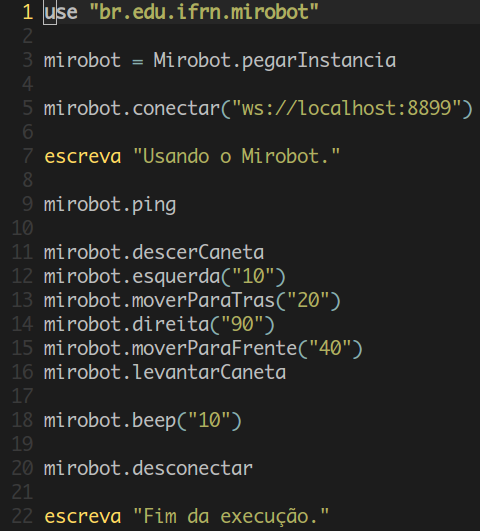
\includegraphics[scale=0.50]{imagens/teste-potigol.png} 
\label{fig:testepotigol}
\end{figure}


	% Capitulo 4: Quarto cap���tulo (arquivo Includes/Capitulo4.tex)
%	% Cap�tulo 4
\chapter{Capítulo 4}

\section{Seção 1}

Teste para símbolo

\simb[$\lambda$ (algum símbolo)]{$\lambda$}


\section{Seção 2}

Teste para abreviatura 

\abrv[IFRN -- Instituto Federal do Rio Grande do Norte]{IFRN}

\abrv[DIATINF -- Diretoria Acadêmica de Gestão e Tecnologia da
Informação]{DIATINF}


	% Capitulo 5: Quinto cap���tulo (arquivo Includes/Capitulo5.tex)
	%% % Cap�tulo 5
\chapter{Capítulo 5}

\section{Seção 1}

Seção 1


\section{Seção 2}

Alguns exemplos de citação: 

No trabalho de Paquete \cite{PaquetePhD}, discute-se sobre algoritmos
de busca local estocásticos aplicados a problemas de Otimização Combinatória
considerando múltiplos objetivos. Por sua vez, o trabalho de
\cite{KnowlesBoundedLebesgue}, publicado nos anais do IEEE CEC de 2003, mostra
uma técnica de arquivamento também empregada no desenvolvimento de algoritmos
evolucionários multi-objetivo, trabalho esse posteriormente estendido para um
capítulo de livro dos mesmos autores \cite{KnowlesBoundedPareto}. Por fim, no
relatório técnico de \citeonline{Jaszkiewicz}, fala-se sobre um algoritmo
genético híbrido para problemas multi-critério, enquanto no artigo de jornal de
Lopez \textit{et al.} \cite{LopezPaqueteStu} trata-se do \textit{trade-off}
entre algoritmos genéticos e metodologias de busca local, também aplicados no
contexto multi-critério e relacionado de alguma forma ao trabalho de Jaszkiewicz
(\citeyear{Jaszkiewicz}).

Outros exemplos relacionados encontram-se em \cite{Silberschatz} (livro),
\cite{DB2XML} (referência da Web) e \cite{Angelo} (Citação de um trabalho).

\subsection{Subseção 5.1}

Subseção 5.1


\subsection{Subseção 5.2}

Subsection 5.2


\section{Seção 3}

Seção 3

	% Consideracoes finais
	% Consideracoes finais
\chapter{Considerações finais}
\label{cap:consideracoes}


As considerações finais formam a parte final (fechamento) do texto, sendo dito
de forma resumida (1) o que foi desenvolvido no presente trabalho e quais os
resultados do mesmo, (2) o que se pôde concluir após o desenvolvimento bem como
as principais contribuições do trabalho, e (3) perspectivas para o
desenvolvimento de trabalhos futuros, como listado nos exemplos de seção abaixo.
O texto referente às considerações finais do autor deve salientar a extensão e
os resultados da contribuição do trabalho e os argumentos utilizados estar
baseados em dados comprovados e fundamentados nos resultados e na discussão do
texto, contendo deduções lógicas correspondentes aos objetivos do trabalho,
propostos inicialmente.


\section{Principais contribuições}



\section{Limitações}



\section{Trabalhos futuros}

Criar um Shell tipo o irb do ruby, facilitar o uso

Extensão para Project Blocks, novas possibilidades para manipulação de objetos tangíveis


	% Bibliografia (arquivo Capitulos/Referencias.bib)
	\bibliography{capitulos/Referencias}
	\bibliographystyle{abnt-alf}

	% Ap���ndice A (arquivo Includes/ApendiceA)
	% Ap�ndice
\apendice
\chapter{Primeiro apêndice}

Os apêndices são textos ou documentos elaborados pelo autor, a fim de
complementar sua argumentação, sem prejuízo da unidade nuclear do trabalho.


	% Anexo A (arquivo Includes/AnexoA)
	% Anexo
\anexo
\chapter{Primeiro anexo}

Os anexos são textos ou documentos não elaborado pelo autor, que servem de
fundamentação, comprovação e ilustração.


	% P���gina em branco
	\newpage

\end{document}
